% ----------------------------------------------------------------------- %
% Arquivo: 2-fundamentacao.tex
% ----------------------------------------------------------------------- %

\chapter{Fundamentação Teórica}
\label{c_fundamentacao}

% ----------------------------------------------------------------------- %
\section{Computação em Nuvem}

Segundo \citeonline{nist}, a computação em nuvem é definida como:

\begin{citacao}
``[...] \textit{um modelo que possibilita acesso através da rede a recursos (por exemplo, redes, servidores, armazenamento, aplicações e serviços) de forma universal, conveniente e sob demanda, que podem ser rapidamente fornecidos e escaláveis com baixo esforço e interação com o provedor do serviço. De acordo com as necessidades e limitações do sistema, nuvens podem ser implantadas de forma privada, pública, híbrida e comunitária. Este modelo de computação é composto de cinco características essenciais, quatro modelos de implantação e três modelos de serviço}.''
\end{citacao}

As características, modelos de implantação e modelos de serviços estão descritos a seguir.

\subsection{Características Essenciais}

\begin{itemize}
    \item Autoatendimento sob demanda: um usuário da nuvem pode utilizar recursos computacionais sob demanda sem necessidade de intervenção do provedor dos serviços \cite{public2};
    \item Amplo acesso a rede: recursos estão disponíveis através da rede e podem ser acessados através de mecanismos padronizados por plataformas heterogêneas (dispositivos móveis, \textit{tablets} e \textit{laptops}, por exemplo) \cite{nist};
    \item \textit{Pooling} de recursos: os recursos computacionais da nuvem são localizados conjuntamente (seja geograficamente ou virtualmente) em um esforço para servir múltiplos usuários, sem que os usuários tenham conhecimento sobre onde os dados estão de fato armazenados \cite{pooling};
    \item Elasticidade rápida: recursos podem ser rapidamente alocados e liberados, sendo que para usuários a capacidade de alocação de recursos geralmente aparenta ser ilimitada a qualquer momento \cite{nist};
    \item Serviços mensuráveis: sistemas em nuvem automaticamente controlam e otimizam recursos ao mensurar e abstrair recursos utilizados por serviços (armazenamento, banda, número de usuários ativos, entre outros). A utilização de recursos pode ser monitorada, controlada e informada, provendo transparência tanto para provedor do serviço quanto para o usuário \cite{nist}.
\end{itemize}

\subsection{Modelos de Implantação}

Nuvens de computação podem ser implementadas de quatro formas distintas, seguindo o modelo de nuvens públicas, privadas, híbridas ou comunitárias.

Em uma nuvem pública os serviços são acessíveis através da \textit{Internet} e disponibilizados por um provedor de serviço, responsável por manter e gerenciar a infraestrutura da nuvem e manter o serviço \cite{public2}. Estes serviços podem incluir uma variedade de aplicações ou serviços de armazenamento, por exemplo. Exemplos de serviços de processamento fornecidos em nuvens públicas são a \textit{Microsoft Azure Servires Platform}, a \textit{Amazon Elastic Compute Cloud} e a \ac{GCP} \cite{sdn}.

Ao contrário de nuvens públicas, as nuvens privadas são reservadas para uso exclusivo de uma única organização \cite{public2}. Esta nuvem pode ser mantida, gerenciada e operada pela organização, terceiros, ou uma combinação de ambos, e pode existir dentro ou fora das premissas da organização \cite{nist}.

Em nuvens híbridas a infraestrutura da nuvem é composta por duas ou mais infraestruturas de nuvens distintas (privadas, comunitárias ou públicas) que continuam sendo entidades separadas, mas são associadas por padronizações ou tecnologias proprietárias que permitem portabilidade de dados ou aplicações \cite{nist}. 

No modelo de nuvens comunitárias a infraestrutura da nuvem é fornecida para uso exclusivo de uma comunidade específica de usuários de organizações que compartilhem valores, políticas, missões ou requisitos de segurança. Ela pode ser mantida, gerenciada e operada por uma ou mais organizações da comunidade, terceiros, ou uma combinação de ambos, e pode existir dentro ou fora da organização \cite{nist}.

\subsection{Modelos de Serviço}

Três são os modelos de serviços de nuvens, que procuram atender a necessidades distintas. Estes modelos são exibidos na \autoref{service_models} e explicados a seguir.

O modelo de \ac{SaaS} é uma forma de computação em nuvem onde o usuário acessa e utiliza aplicações remotas. Como exibido na \autoref{service_models}, o usuário geralmente não possui acesso ao sistema operacional do servidor e não é responsável por manter o serviço, utilizando assim apenas as funcionalidades das aplicações \cite{servicemodels}.

Já no modelo de serviço \ac{PaaS} o provedor do serviço fornece a usuários uma plataforma de computação (geralmente virtual) que provê sistemas operacionais prontos para execução \cite{servicemodels}. O usuário não controla ou gerencia a infraestrutura física da nuvem (como rede, servidores ou armazenamento), mas possui controle sobre as aplicações instaladas e configurações destas aplicações \cite{nist}.

O terceiro modelo, amplamente utilizado no desenvolvimento de aplicações e serviços em nuvem, é o de \ac{IaaS}. No \ac{IaaS} o usuário não controla ou gerencia a infraestrutura física, mas possui controle sobre sistemas operacionais, armazenamento e aplicações, e \textbf{possivelmente} controle limitado sobre componentes de rede (como \textit{firewalls}, por exemplo) \cite{nist}. Sistemas operacionais e aplicações são passíveis de administração pelo usuário, e é de sua responsabilidade a manutenção desses sistemas \cite{servicemodels}.  

Já no modelo de infraestrutura privada o administrador do sistema é responsável por manter todas as camadas, desde a parte física , como servidores e armazenamento, quanto de \textit{software}, como sistema operacional e aplicações.

\begin{figure}[!htpb]
	\centering
	\caption{Modelos de serviço em nuvem}
    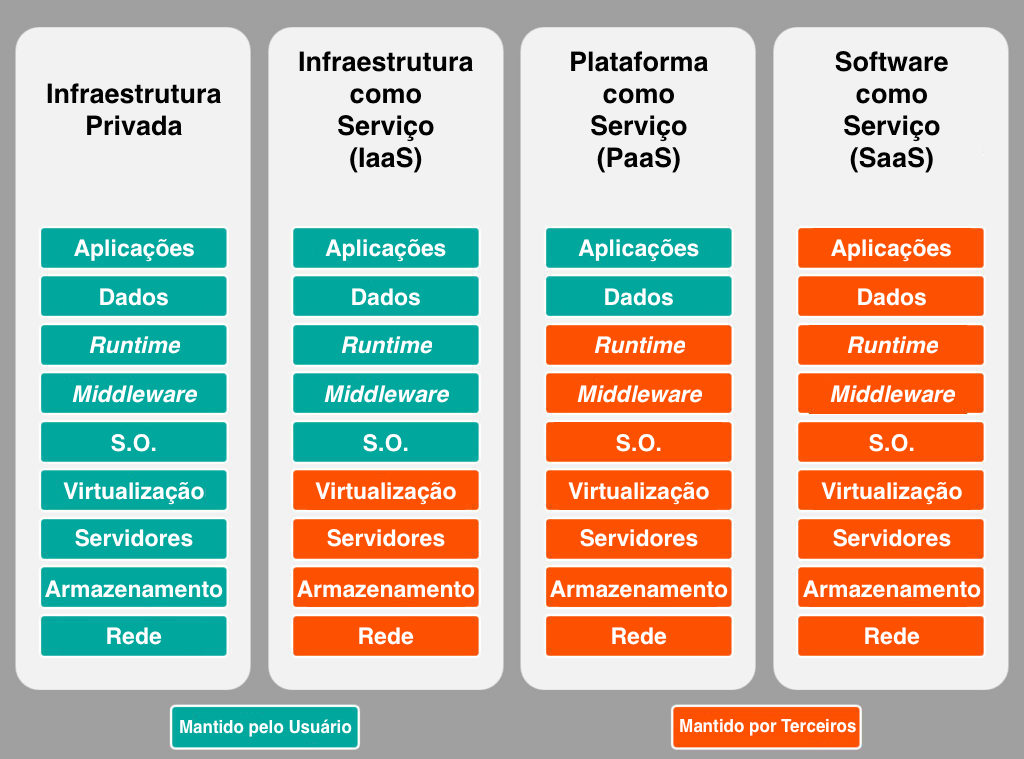
\includegraphics[width=14cm]{TCC/figuras/2-fundamentacao/ServiceModels}
    
	Fonte: Traduzido de \cite{servicemodelsimage}
 	\label{service_models}
\end{figure}

% ----------------------------------------------------------------------- %
\section{Sistemas Distribuídos}

De acordo com \citeonline{tanenbaum}, um sistema distribuído é um conjunto de computadores independentes que se apresenta a seus usuários como um sistema único e coerente. Entre as vantagens na utilização de sistemas distribuídos destacam-se a escalabilidade e redundância do sistema, que permitem que o sistema atenda à diversas aplicações e usuários. A contrapartida é a complexidade em seu gerenciamento, haja vista que o gerenciamento de recursos e dimensão do sistema ficam mais complexos.

Para que o sistema se apresente ao usuário como um sistema distribuído é necessário que ele cumpra quatro metas fundamentais \cite{tanenbaum}:

\begin{itemize}
    \item Acesso a recursos: o acesso a recursos do sistema deve ser eficiente e seguro.
    \item Transparência da distribuição: o sistema deve se apresentar ao usuário sendo como um único sistema, mesmo estando distribuído entre diversos computadores (por exemplo, ao acessar uma página \textit{Web} o usuário não possui conhecimento sobre qual servidor está de fato acessando).
    \item Abertura: ``um sistema distribuído aberto é um sistema que oferece serviços de acordo com regras padronizadas que descrevem a sintaxe e semântica desses serviços''  \cite{tanenbaum}.
    \item Escalabilidade: um sistema distribuído pode ser escalável em relação a seu tamanho (com adição de usuários e recursos ao sistema), termos geográficos (usuários e recursos podem estar longes uns dos outros) e administrativos (facilidade de gerenciamento) \cite{tanenbaum}.
\end{itemize}

Sistemas de computação distribuídos são classificados em dois subgrupos, sendo estes subgrupos os sistemas de computação em \textit{cluster} e em \textit{grid} \cite{tanenbaum}. Um \textit{cluster} consiste em um conjunto de computadores de \textit{hardware} semelhante interconectados entre si por uma rede de alta velocidade e que trabalham conjuntamente para executar tarefas que requerem alto poder computacional \cite{cluster&grid}. Já na computação em \textit{grid} o \textit{hardware} das estações é heterogêneo e as estações que compõem o sistema podem ser de diferentes organizações \cite{tanenbaum}. Em sistemas de computação em \textit{grid} a estratégia empregada para coordenação entre as estações é a utilização de um \textit{middleware} que divide e distribui tarefas entre os computadores \cite{cluster&grid}.

Como é possível perceber, é necessário que os computadores que fazem parte do sistema distribuído estejam altamente coordenados para realizar a computação de forma eficiente. Diversos modelos de coordenação são utilizados, como o Linda, o \textit{publish/subscribe} e o Jini \cite{tanenbaum2}. 

\subsection{Virtualização de Sistemas Operacionais}

Com o crescimento de volumes de dados e de serviços fornecidos através de redes \ac{IP} têm se evidenciado que a virtualização de infraestruturas provê melhor flexibilidade, custo, escalabilidade, utilização de recursos e eficiência energética em \textit{data centers} \cite{bari}. Até recentemente, a virtualização neste contexto significava apenas virtualização em \textit{hardware} através da execução de máquinas virtuais \cite{tay}, apesar do conceito de virtualização ser discutido e pesquisado há mais de 40 anos \cite{pearce}. Segundo \citeonline{walters}, a virtualização de sistemas operacionais pode ser majoritariamente categorizada em quatro grupos: virtualização total ou completa,  paravirtualização, virtualização em nível de sistema operacional e virtualização assistida por \textit{hardware}. Estes tipos de virtualização são explicados a seguir.

\subsubsection{Tipos de Virtualização de Sistema Operacional}

\begin{itemize}
    \item Virtualização total ou completa (\textit{Full Virtualization}): Também chamada de emulação de \textit{hardware}. Nesta categoria, o \textit{hypervisor} (\textit{software}, \textit{firmware} ou \textit{hardware} que encapsula e roda o sistema operacional emulado) provê as mesmas entradas, saídas e comportamentos que seriam esperados de um \textit{hardware} específico \cite{pearce}. De forma simples, o sistema operacional emulado não possui conhecimento de que está sendo virtualizado, e sim de que está sendo executado diretamente em \textit{hardware}. Este tipo de virtualização é computacionalmente intensivo e possui alto custo, pois o sistema operacional emulado não possui conhecimento de que está na verdade acessando um \textit{hardware} emulado pelo \textit{hypervisor}, o qual captura as exceções de acesso ao \textit{hardware} do sistema emulado e as emula de acordo com as configurações do \textit{hardware} emulado;
    \item Paravirtualização (\textit{Paravirtualization}): Na paravirtualização propõe-se que o sistema operacional virtualizado saiba que está sendo executado na camada virtual e interaja com a mesma. Isso implica a alteração do sistema operacional virtualizado, mas garante uma grande cooperação entre as duas camadas \cite{grosmann};
    \item Virtualização em nível de Sistema Operacional (\textit{Operating System-level Virtualization}): De forma simples, esta técnica de virtualização permite que recursos possam ser isolados dentro de um sistema operacional para execução de instâncias de espaços de usuários e aplicações, sendo o gerenciamento destes recursos realizados pelo sistema operacional, e não por um \textit{hypervisor}, o que aumenta o desempenho dessas instâncias \cite{walters};
    \item Virtualização Assistida por \textit{Hardware} (\textit{Hardware-Assisted Virtualization}): Esta técnica de virtualização consiste em uma virtualização total mas com auxílio em \textit{hardware} do processador, permitindo que as instruções da máquina virtual não sejam executadas em um processador emulado pelo \textit{hypervisor}, e sim diretamente no processador da máquina real \cite{walters}.
\end{itemize}

\subsection{Virtualização de Redes}

A virtualização de servidores sozinha não é suficiente para resolver os problemas e limitações de grandes infraestruturas, tais como os riscos de segurança ocasionados pela não-restrição de protocolos de comunicação utilizados por máquinas reais, as quais podem estar executando diversas máquinas virtuais simultaneamente \cite{bari}. Neste contexto, técnicas de virtualização de rede também têm sido aplicadas com o objetivo de solucionar alguns destes problemas e melhorar a performance e segurança do sistema. Técnicas como a utilização de \ac{VLANs} são as mais tradicionais em termos de virtualização, pois permitem que sejam criadas redes locais virtuais, restringindo assim o domínio de \textit{broadcast} de cada dispositivo e possibilitando a resolução de diversos dos problemas de \textit{data centers} \cite{bari}.
Com a utilização de técnicas de virtualização de rede torna-se fundamental a organização de uma topologia que facilite a implementação e manutenção da rede. Ao definir a topologia de uma rede, é importante definir se ela será escalável horizontalmente ou verticalmente. A escalabilidade horizontal refere-se a adicionar nós no sistema, o que permite a distribuição de carga de trabalho a múltiplas máquinas e a utilização de \textit{hardware} heterogêneo no sistema \cite{gregol}. Já a escalabilidade vertical refere-se a melhorar o sistema ao adicionar mais recursos a um nó, tais como aumentar a memória ou capacidade de armazenamento do mesmo \cite{barzu}. A \autoref{datacenter_topology} exibe a topologia convencional de \textit{data center} segundo \citeonline{barzu}.

\begin{figure}[!htpb]
	\centering
	\caption{Topologia convencional de um \textit{data center}}
    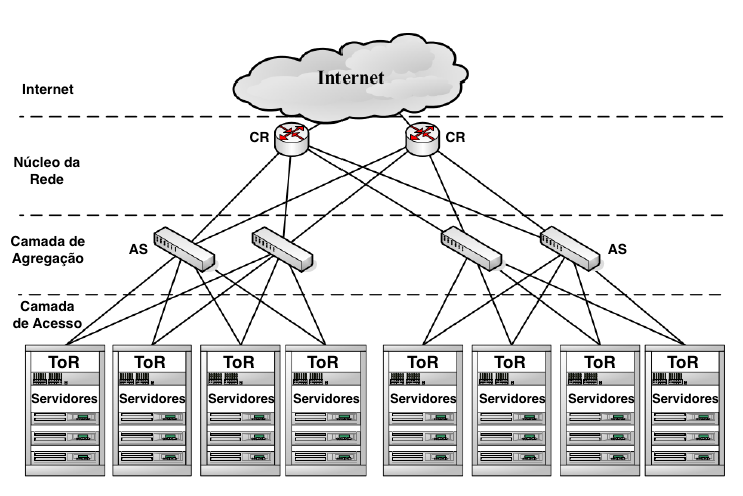
\includegraphics[width=13cm]{TCC/figuras/2-fundamentacao/DCNetworkConventional}
    
	Fonte: Traduzido de \cite{bari}
 	\label{datacenter_topology}
\end{figure}

Como exibido na \autoref{datacenter_topology}, esta topologia é convencionalmente horizontal, pois permite que diferentes dispositivos de uma mesma categoria (\textit{switches}, roteadores e servidores) sejam adicionados ao sistema, evitando assim a necessidade de utilizar tecnologias proprietárias e altos custos na melhoria do sistema, por exemplo. É importante ressaltar que nem sempre esta solução é a ideal, pois ocorrem casos em que melhorar um nó individual é mais efetivo do que adicionar nós ao sistema. Por exemplo, pode ser mais efetivo melhorar a capacidade de processamento de um nó para fornecimento de um serviço específico do que adicionar nós ao sistema. Na topologia apresentada na \autoref{datacenter_topology}, o \textit{switch} \ac{ToR} realiza a conexão entre os servidores montados em um mesmo \textit{rack}, enquanto os \textit{switches} de agregação (\ac{AS}) encaminham o tráfego dos \textit{switches} \ac{ToR} para os roteadores do núcleo da rede (\ac{CR}) \cite{bari}. É importante ressaltar a redundância entre os \textit{switches} \ac{ToR} e de agregação, que garantem que o sistema continuará em operação em caso de falhas pontuais. Esta topologia é denominada topologia \ac{ToR} (referenciando o \textit{switch} \ac{ToR}, componente vital do sistema).

\subsection{Contêineres}

Os avanços no \textit{kernel} do Linux levaram ao desenvolvimento de isolamento de recursos baseado em contêineres \cite{containersXvms}. De forma simples, um contêiner pode ser definido como um pacote executável de um \textit{software} que inclui tudo o que é necessário para executar este \textit{software}: código, bibliotecas, configurações, ferramentas, entre outros \cite{aboutcontainer}. 

Contêineres e máquinas virtuais são soluções distintas para problemas distintos. De acordo com \citeonline{paascontainer}:

\begin{citacao}
``[...] \textit{contêineres são ferramentas para prover software - isto é, seu foco é na entrega de uma PaaS - com grande portabilidade e interoperabilidade enquanto utilizando técnicas de virtualização. Por outro lado, máquinas virtuais se preocupam com alocação e gerenciamento de hardware - isto é, seu foco é na entrega de uma IaaS que fornece serviços através da virtualização de hardware}.''
\end{citacao}

Existem diferentes tecnologias de contêineres, sendo o Docker uma das tecnologias que está se tornando uma das mais utilizadas para criação de contêineres \cite{openstackContainer}. O Docker é uma ferramenta que facilita a criação e distribuição de contêineres com suas dependências \cite{containers&docker}, sendo um projeto de código aberto que possui mais de 3 mil colaboradores \cite{aboutdocker}. A \autoref{virtualization_layers} exibe a abstração das camadas de máquinas virtuais e contêineres Docker. É possível perceber que, diferentemente de máquinas virtuais, contêineres não requisitam que seja realizada a virtualização completa de um sistema operacional. A vantagem desta abordagem é de que não há duplicação de funcionalidades, como por exemplo chamadas de \textit{hardware}, já que apenas um sistema operacional lida com todo o acesso ao \textit{hardware} \cite{containers&docker}.

\begin{figure}[!htpb]
	\centering
	\caption{Comparação entre máquinas virtuais e contêineres}
    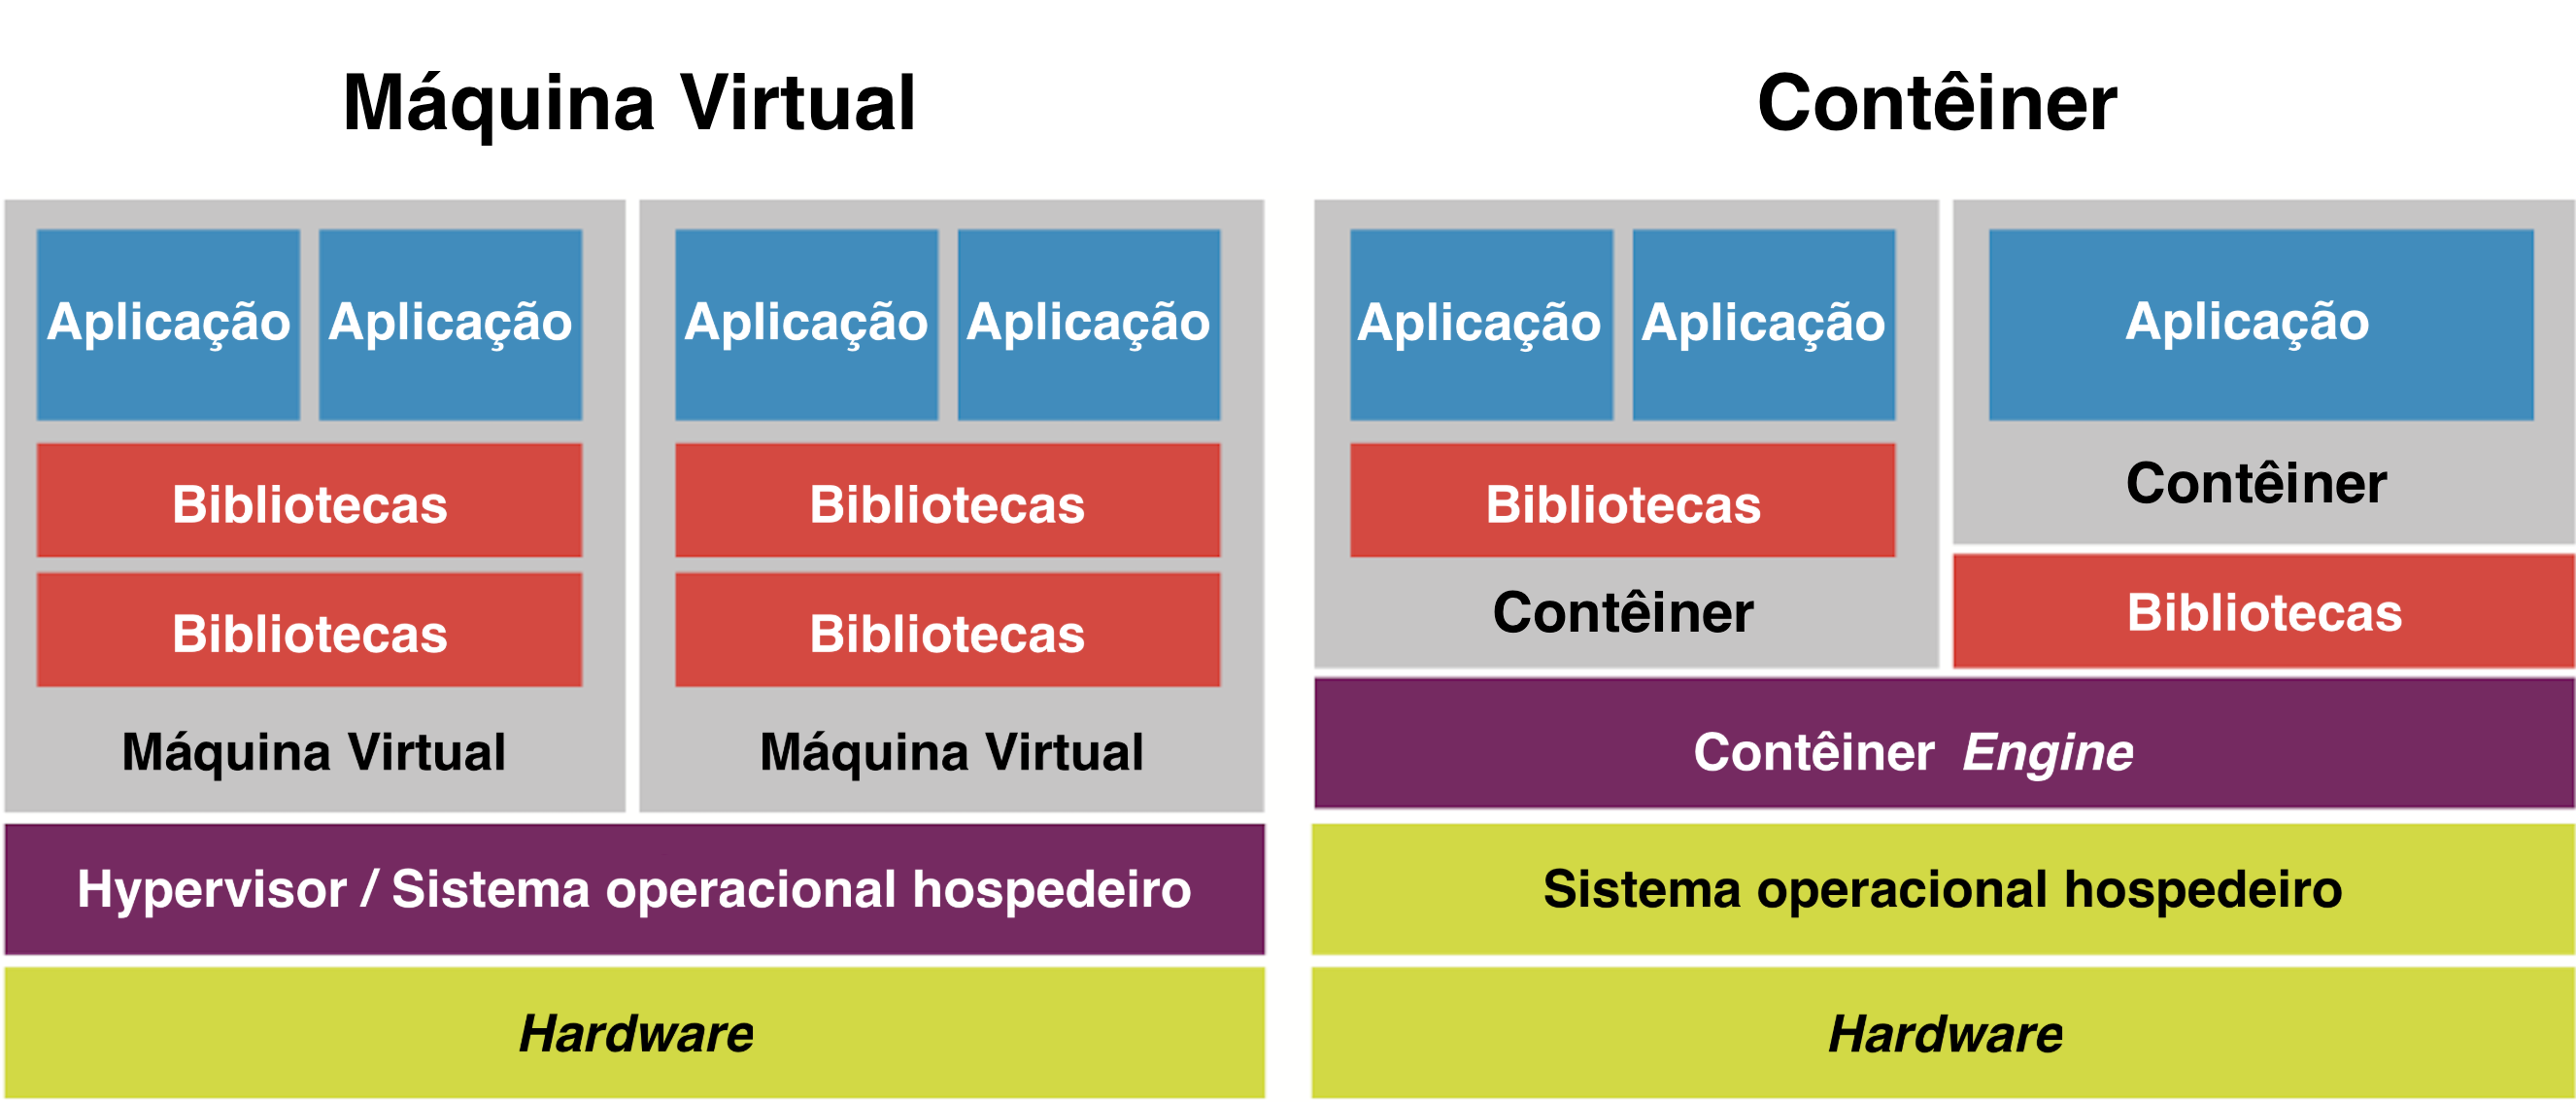
\includegraphics[width=13cm]{TCC/figuras/2-fundamentacao/Virtualization}
    
	Fonte: Traduzido de \cite{paascontainer}
 	\label{virtualization_layers}
\end{figure}

Como contêineres - diferentemente de máquinas virtuais - rodam como processos em um mesmo sistema operacional, é possível (e necessário) restringir e limitar o acesso a recursos do sistema operacional hospedeiro. Para contêineres em Linux, o controle ao acesso de recursos é realizado através de \textit{namespaces} e grupos de controle (\textit{cgroups}) \cite{containers&docker}. \textit{Namespaces} permitem que grupos de processos sejam separados, evitando assim que estes processos acessem recursos de outros grupos \cite{paascontainer}. Grupos de controle permitem o gerenciamento de recursos por grupos de processos, possibilitando que o uso de memória seja limitado para um grupo, por exemplo \cite{paascontainer}.

Segundo \citeonline{containersXvms}, quatro são as características que tornam contêineres úteis e atrativos no desenvolvimento de aplicações e fornecimento de serviços:

\begin{itemize}
    \item Portabilidade: aplicações podem ser desenvolvidas em um ambiente e ser implantadas em diversos outros ambientes sem necessidade de alterar o contêiner.
    \item Rapidez na entrega da aplicação: o fluxo de desenvolvimento de contêineres permite que administradores de sistema, desenvolvedores e equipe de testes efetuem a implantação da aplicação rapidamente, pois apenas os desenvolvedores precisam se preocupar com o formato e conteúdo do contêiner e os administradores de sistema com sua implantação nos servidores.
    \item Escalabilidade: a escalabilidade vertical e horizontal de contêineres 
    é muito mais rápida do que a de máquinas virtuais, já que os recursos utilizados pelos contêineres são oferecidos nativamente pelo sistema operacional, sem necessidade de virtualização de chamadas de \textit{hardware}.
    \item Maior carga de trabalho e densidade: como não é necessário utilizar um \textit{hypervisor} para virtualização, é possível executar uma quantidade maior de contêineres do que de máquinas virtuais concorrentemente. Além disso, o processamento está concentrado na aplicação, sem necessidade de virtualização de chamadas de \textit{hardware}, como no caso de máquinas virtuais, por exemplo.
\end{itemize}

Após a criação do contêiner, é possível gerenciá-lo utilizando uma ferramenta de orquestração de contêineres, que permite a criação de \textit{clusters} de contêineres e seu gerenciamento.

\subsubsection{Orquestração de Contêineres}

De acordo com \citeonline{containerOrchestration}, uma plataforma de orquestração de contêineres pode ser, de forma geral, definida como um sistema que provê um \textit{framework} para integração e gestão de contêineres em larga escala.  Estas plataformas simplificam a gestão de contêineres e fornecem um \textit{framework} para não apenas realizar a implantação inicial de contêineres mas também a gestão de múltiplos contêineres como uma entidade, seja para propósitos de escalabilidade ou disponibilidade, por exemplo. Como exemplos de orquestradores de contêineres populares pode-se citar o Docker Swarm e o Kubernetes, enquanto  \ac{GKE}, \ac{Amazon EKS} e \ac{AKS} são implementações do orquestrador Kubernetes em nuvens públicas.

\subsubsubsection{Kubernetes}

Kubernetes é uma plataforma de código aberto para orquestração de contêineres a qual facilita tanto configurações declarativas e automatizações. Disponibilizada em 2014 e criada pela Google, hoje a plataforma é mantida pela \ac{CNCF} \cite{aboutkubernetes}.

Um \textit{cluster} Kubernetes consiste em dois tipos de recursos: mestres e nós. A interligação entre estes recursos coordenados por um mesmo orquestrador Kubernetes é denominado \textit{cluster} \cite{minikubeCluster}. Os mestres são responsáveis por coordenar o \textit{cluster}, enquanto os nós são as unidades que de fato executam as aplicações do \textit{cluster}, as quais são implantadas através de contêineres. A \autoref{k8sArchitecture} mostra a arquitetura básica de um \textit{cluster} Kubernetes.

\begin{figure}[!htpb]
	\centering
	\caption{Arquitetura de \textit{cluster} Kubernetes}
    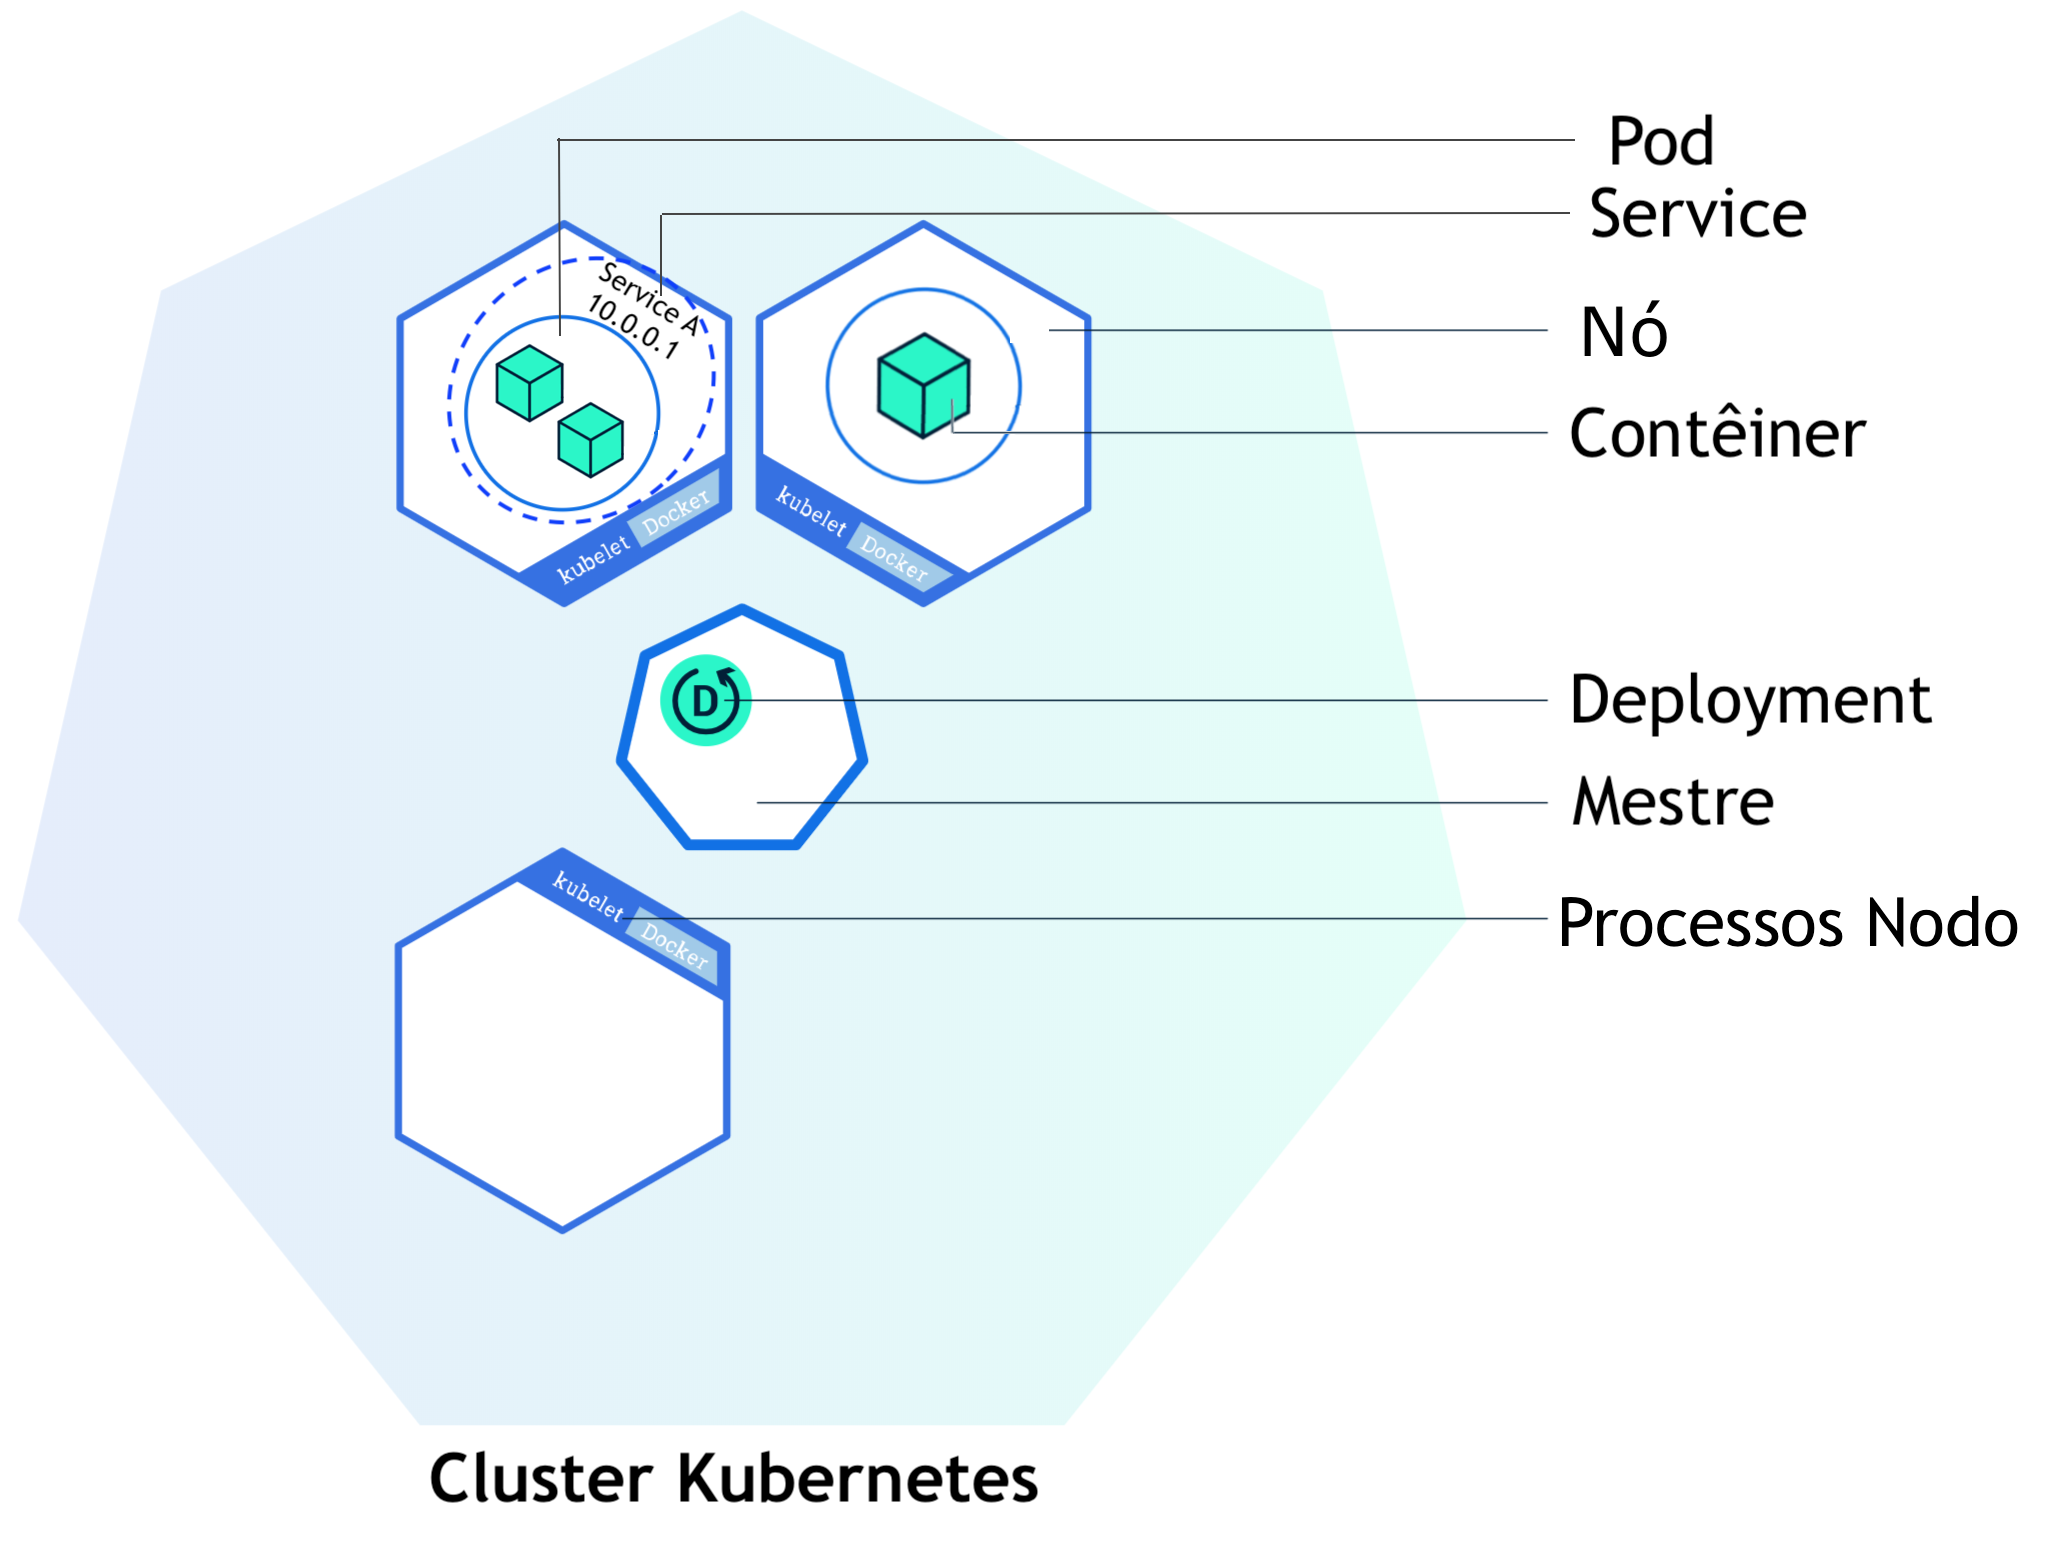
\includegraphics[width=13cm]{TCC/figuras/2-fundamentacao/K8s-architecture}
    
	Fonte: Adaptado de \cite{minikubeCluster}
 	\label{k8sArchitecture}
\end{figure}

Na aquitetura da \autoref{k8sArchitecture} há um mestre e três nós. Os \textit{pods}, \textit{deployments} e \textit{services} são entidades persistentes do sistema Kubernetes e são tratados como objetos \cite{kubernetesObjects}. Já o processo \textit{kubelet} é o ``agente'' que roda no nó para que este faça parte do \textit{cluster} \cite{kubernetesKubelet}.

Um \textit{pod} é um grupo de um ou mais contêineres que compartilham armazenamento, rede e outros recursos computacionais e especifica como executar estes contêineres. Assim como contêineres, \textit{pods} são isolados através da utilização de \textit{namespaces} linux, \textit{cgroups} e outras formas de isolamento. \textit{Pods} podem ser utilizados para implantar \textit{proxies} e ferramentas de monitoramento, por exemplo \cite{kubernetesPods}.

\textit{Services} são uma abstração que definem as políticas de acesso a \textit{pods}. \textit{Pods} podem ser expostos através de diferentes tipos de \textit{services}, havendo desde \textit{services} que expõem uma porta do nó externamente ao \textit{cluster} (\texttt{NodePort}) até \textit{services} que limitam o acesso ao \textit{pod} a endereços \ac{IP} internos ao \textit{cluster} (\texttt{clusterIP}) \cite{kubernetesServices}.

Já um \textit{deployment} permite que \textit{pods} sejam criados e atualizados através de linguagem declarativa. \textit{Deployments} fornecem um mecanismo de auto-reparação que permite que \textit{pods} sejam reiniciados caso falhas ocorram, por exemplo \cite{kubernetesDeployments}.

Outros componenentes do Kubernetes que também merecem destaque são o \textit{StorageClass} e o \textit{Ingress}. De forma simples, uma \textit{StorageClass} é uma classe que descreve como o armazenamento através de volumes persistentes (\ac{PV}) será provido a aplicações \cite{kubernetesStorageClass}. Esta abordagem é vantajosa pois permite que diferentes \textit{StorageClasses} com diferentes características possam ser criados no \textit{cluster} Kubernetes, permitindo assim que a aplicação utilize a que melhor se adeque as suas necessidades. Para utilização de um volume é necessário que um \textit{pod} solicite a criação deste volume através de uma requisição de volume persistente (\ac{PVC}), a qual será processada pelo \textit{Storage Class}.

Já o \textit{Ingress} é um recurso do Kubernetes que atua na camada de aplicação da arquitetura \ac{TCP}/\ac{IP} e permite a criação de regras de acesso a serviços do \textit{cluster} através de domínios ou recursos personalizados, além de também possibilitar o balanceamento de carga e implementação de criptografia no acesso a estes serviços. Um \textit{Ingress} consiste, portanto, de um conjunto de regras que permitem que o tráfego de entrada possa acessar os serviços do \textit{cluster} \cite{kubernetesIngress}. É importante ressaltar que aprimoramentos estão sendo realizados para possibilitar que a camada de transporte também seja controlada através do \textit{Ingress}, mas esta funcionalidade ainda está em desenvolvimento \cite{ingressTCPUDP}.

Outros objetos, tais como \textit{ReplicaSets} e \textit{ResourceQuotas} também são vastamente utilizados em \textit{clusters} Kubernetes. Também é possível criar definições de recursos customizados (\ac{CRD}) através da \ac{API} do Kubernetes para que novos objetos possam ser utilizados. A \autoref{k8schematic} exemplifica a organização dos objetos \textit{Deployment}, \textit{ReplicaSet}, \textit{Pod}, \ac{PVC}, \ac{PV}, \textit{StorageClass}, \textit{Service} e \textit{Ingress Controller} na implantação de uma aplicação em um \textit{cluster} Kubernetes.

\begin{figure}[!htpb]
	\centering
	\caption{Objetos do Kubernetes}
    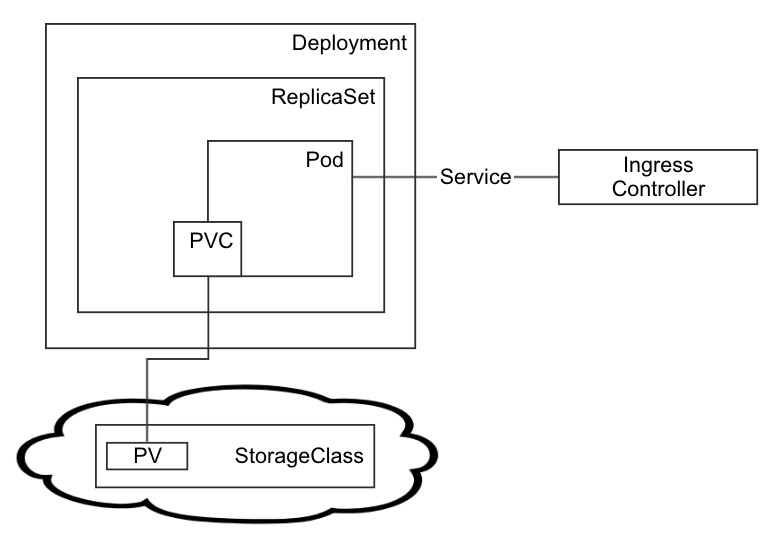
\includegraphics[width=13cm]{TCC/figuras/2-fundamentacao/k8s-complete-schematic.png}
    
	Fonte: Elaborado pelo autor.
 	\label{k8schematic}
\end{figure}

\subsubsubsection{Helm}

O Helm é um gerenciador de pacotes para Kubernetes \cite{abouthelm}. Estes pacotes são denominados \textit{charts} e podem ser instalados em um \textit{cluster} Kubernetes a partir de repositórios públicos ou privados, dispensando assim a necessidade de criar todos os recursos necessários para a implantação de uma aplicação manualmente.

Um \textit{chart} Helm pode, por exemplo, implantar uma aplicação WordPress em um \textit{cluster} de forma automatizada, criando de forma automatizada os \textit{Deployments}, \textit{Services} e \textit{ReplicaSets} necessários para implantacão da aplicação.

\subsubsection{Rancher}

Assim como o Kubernetes é uma ferramenta para orquestração de contêineres, o Rancher é uma plataforma para administração de \textit{clusters} Kubernetes. Ele facilita, por exemplo, o monitoramento dos recursos de \textit{clusters} e criação e manutenção de \textit{clusters} híbridos \cite{rancherOverview}.

A arquitetura em alto nível do Rancher é simples: é necessário apenas a criação de um servidor para gerenciamento dos \textit{clusters} e configurar a conexão e permissões de acesso do Rancher a estes \textit{clusters}. Também é possível utilizar a ferramenta de gerenciamento \ac{RKE} para rápida criação de \textit{clusters} Kubernetes.

% ----------------------------------------------------------------------- %
\section{Sistemas de Arquivos}

De acordo com \citeonline{tanenbaum2}, a parte do sistema operacional que trata do modo como os arquivos são estruturados, nomeados, acessados, usados, protegidos e implementados é o sistema de arquivos. Exemplos de sistemas de arquivos são o ISO 9660 (utilizado em CD-ROMs), FAT-32 (extensão do sistema de arquivos MS-DOS da Microsoft) e EXT4 (evolução do sistema de arquivos EXT3 do Linux). 

\subsection{Sistemas de Arquivos Distribuídos}

Segundo \citeonline{authdfs}, um sistema de arquivos distribuído é um sistema no qual os arquivos estão armazenados e distribuídos em computadores diferentes interligados por meio de uma rede de comunicação. Um sistema de arquivos distribuído apresenta o mesmo conceito de um sistema de arquivos local, ou seja, ele também trata do gerenciamento de arquivos, porém no contexto distribuído. Ele permite, portanto, que usuários e programas remotos leiam e escrevam dados que estão aparentemente armazenados na máquina do usuário, mas que na verdade estão disponíveis remotamente. Isto significa, portanto, que ele cumpre a meta fundamental de ser um sistema transparente ao usuário.

Além das vantagens inerentes de rápida escalabilidade e maior redundância do sistema distribuído, sistemas de arquivos distribuídos também podem oferecer a vantagem de fornecer acesso a uma base unificada de dados aos usuários, evitando réplicas desnecessárias de arquivos em máquinas locais. Entretanto, uma desvantagem que merece destaque na utilização de sistemas de arquivos distribuídos é a necessidade de uma boa infraestrutura de rede para suportar o constante tráfego de arquivos, que pode ser ineficiente em uma rede precária e de baixas taxas de transmissão.

Exemplos de sistemas de arquivos distribuídos são o Ceph, GlusterFS, StorageOS, \ac{GFS} e Lustre. Dos exemplos citados apenas o primeiro será objeto de estudo deste trabalho, pois a implementação deste sistema de arquivos em Kubernetes têm recebido grande apoio da \ac{CNCF} \cite{rookincubator}.

\subsubsection{Ceph}

Ceph é um sistema de armazenamento distribuído de código aberto. Este sistema de armazenamento permite que dados sejam armazenados não apenas no formato de arquivos, mas também como blocos e objetos \cite{cephdocumentation}.

O armazenamento através de arquivos ocorre quando os dados são salvos em uma única quantidade de armazenamento, geralmente organizada por diretórios. Já o armazenamento em blocos ocorre quando o armazenamento disponível é dividido em blocos e estes blocos podem ser utilizados por diferentes aplicações, seja de forma distribuída ou não. Finalmente, o armazenamento através de objetos é uma estrutura horizontal onde dados são armazenados como uma unidade denominada objeto e possuem um identificador único que localiza este objeto na estrutura de dados. Este identificador é salvo em um servidor de metadados, que também pode armazenar informações como data de criação do objeto e permissões de acesso, por exemplo \cite{redhatStorage}.

O Ceph foi projetado sob a premissa de que grandes sistemas de armazenamento de dados possuem o potencial de armazenar ainda mais informações, e falhas de componentes não são exceções, e sim constantes \cite{cephFailures}. Assumir que falhas de componentes são comuns no sistema e trabalhar para contornar estas falhas torna o Ceph um sistema poderoso.

Uma das características mais interessantes do Ceph é o algoritmo \ac{CRUSH}. O \ac{CRUSH} é um algoritmo de locação pseudo-randômico que permite que clientes possam computar a localização de um dado no \textit{cluster} sem precisar consultar uma tabela central que guarde a localização de todos os dados do \textit{cluster}. Como consequência, o Ceph busca garantir a escalabilidade e confiabilidade do sistema através da computação inteligente dos dados nele armazenados \cite{cephPerformance}.

Cinco são os componentes principais de um \textit{cluster} Ceph: \ac{OSD}s, \textit{Monitors}, \textit{Managers}, \ac{MDS} e \ac{RADOS}. Cada um destes componentes é explicado a seguir:

\begin{itemize}
    \item \ac{OSD}s: um \ac{OSD} armazena dados, processa replicação de dados e fornece informações de monitoramento para os \textit{Monitors} e \textit{Managers} \cite{aboutceph}. Estes são os componentes de ``mais baixo nível'' do \textit{cluster} Ceph.
    \item \textit{Monitors}: mantém mapas e informações do \textit{cluster}, tais como mapa de outros \textit{Monitors}, \ac{OSD}s e \textit{Managers} existentes, além do mapa \ac{CRUSH} utilizado para computação da localização dos dados armazenados \cite{aboutceph}. \textit{Monitors} também são responsáveis pela autenticação de clientes e \textit{daemons}. Quando um cliente deseja armazenar ou acessar dados do \textit{cluster} ele deve se conectar ao \textit{Monitor} para se autenticar e obter o mapa do \textit{cluster} e, após ser devidamente autenticado, ele poderá conectar-se diretamente o \ac{OSD} correspondente para realizar a operação desejada \cite{cephArchitecture}.
    \item \textit{Managers}: os \textit{Managers} são responsáveis por registrar métricas de execução e estado do \textit{cluster} Ceph, além da carga de trabalho do sistema. Os \textit{Managers} permitem a consulta de métricas do sistema através de \textit{plugins} como uma \textit{dashboard} (painel de controle) e uma \ac{REST} \ac{API} \cite{aboutceph}.
    \item \ac{MDS}s: armazenam metadados do sistema de arquivos Ceph, como permissões e propriedades de arquivos, ou seja, se o Ceph for utilizado como armazenamento em blocos ou objetos \ac{MDS}s não serão necessários \cite{aboutceph}.
    \item \ac{RADOS}: consiste na junção de \ac{OSD}s e \textit{Monitors} para distribuição de dados como objetos pelo \textit{cluster} e replicação de dados \cite{openstackCephBlock}. O \ac{RGW} é uma interface que fornece uma \ac{REST} \ac{API} para acesso aos objetos armazenados pelo \ac{RADOS}. Esta \ac{API} é compatível com as interfaces S3 da Amazon e OpenStack Swift \cite{cephRadosGW}.
\end{itemize}

\subsubsection{Rook}

O Rook é um projeto de código aberto incubado pela \ac{CNCF} \cite{rookincubator}. De forma simples, o Rook é um orquestrador de armazenamento para \textit{clusters} Kubernetes que automatiza a implantação do Ceph nestes sistemas. No presente momento (segundo semestre de 2018) a implementação do Ceph através do Rook está em estado Beta \cite{rookdocumentation}.

O Rook permite, por exemplo, que sejam automaticamente implantados todos os \ac{OSD}s necessários em nodos específicos, dispensando assim a necessidade de manualmente instalar e configurar os \textit{daemons} necessários nestes nodos. Assim como o Ceph, é possível utilizar o Rook para orquestrar o armazenamento de dados através de arquivos, blocos e objetos.

O armazenamento através de blocos pode ser empregado no Rook através da implantação de uma \textit{Storage Class} do Rook via \ac{CRD}. Já o armazenamento de objetos pode ser realizado através de uma \textit{Object Store}, a qual - assim como o \ac{RADOS} do Ceph - oferece uma \ac{REST} \ac{API} para acesso aos objetos armazenados. Já um sistema de arquivos distribuído pode ser implantado no Rook através de um \textit{Shared File System}, o qual também pode ser associado a serviços como um volume.

A maior parte dos componentes criados pelo Rook no \textit{cluster} são componentes equivalentes aos do Ceph. Um \textit{pod} \ac{OSD} do Rook, por exemplo, também possui como função armazenar os dados em disco e prover acesso a estes dados para outros programas.


\subsection{Convergência de infraestrutura}

Uma \ac{CI} é a convergência das infraestruturas de computação, armazenamento e rede em um \textit{data center} \cite{netappconvergence}. A \ac{CI} almeja alcançar o melhor desempenho do sistema com padronização dos protocolos e \textit{hardware} utilizado no \textit{data center}, muitas vezes através da utilização de \textit{hardware} proprietário que realize funções específicas \cite{netappconvergence}.
 
Uma \ac{HCI} é uma infraestrutura definida por \textit{software} que pode ser dimensionada horizontalmente \cite{vmwarehyperconvergence} e que combina computação, virtualização, armazenamento e rede em um único \textit{cluster} \cite{ciscohyperconvergence}. A hiperconvergência traz simplicidade a \textit{clusters} locais com uma única e simples plataforma de computação e gerenciamento. Com a \ac{HCI}, todas as principais funções do \textit{data center} são executadas em uma camada de \textit{software} altamente integrada, simplificando o fornecimento de serviços que antes exigiam \textit{hardware} específico para uma finalidade. Dentre as vantagens oferecidas pela hiperconvergência encontram-se a simplicidade de administração do sistema e o baixo custo total de propriedade \cite{vmwarehyperconvergence}. Como a proposta de uma infraestrutura hiperconvergente consiste na combinação das infraestruturas de computação, virtualização, armazenamento e rede em um único \textit{cluster}, é possível alcançar este modelo através de uma infraestrutura de contêineres, que pode combinar todas as infraestruturas através de uma única plataforma de gerenciamento. A \autoref{hcischematic} mostra que armazenamento, rede e computação podem ser combinados através da utilização de contêineres, sendo o armazenamento implementado através do \textit{StorageClass}, a rede através de \textit{Services} e recursos \textit{Ingress} (gerenciados pelo \textit{Ingress Controller}) e a computação através dos \textit{Pods}, \textit{Deployments} e \textit{ReplicaSets}.

\begin{figure}[!htpb]
	\centering
	\caption{Infraestrutura hiperconvergente de contêineres}
    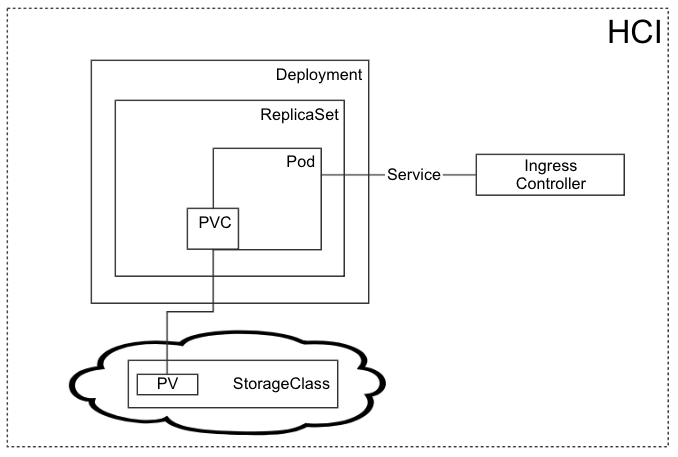
\includegraphics[width=11cm]{TCC/figuras/2-fundamentacao/hci-container.png}
    
	Fonte: Elaborado pelo autor.
 	\label{hcischematic}
\end{figure}